\hypertarget{group__xEventGroupCreate}{}\section{x\+Event\+Group\+Create}
\label{group__xEventGroupCreate}\index{x\+Event\+Group\+Create@{x\+Event\+Group\+Create}}
Collaboration diagram for x\+Event\+Group\+Create\+:\nopagebreak
\begin{figure}[H]
\begin{center}
\leavevmode
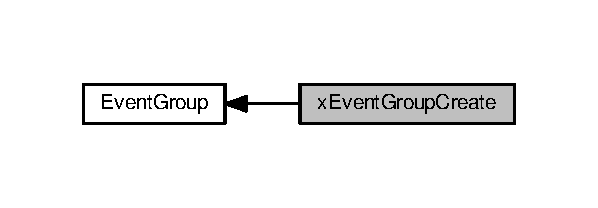
\includegraphics[width=287pt]{df/d78/group__xEventGroupCreate}
\end{center}
\end{figure}
\hyperlink{event__groups_8h}{event\+\_\+groups.\+h} 
\begin{DoxyPre}
EventGroupHandle\_t xEventGroupCreate( void );
\end{DoxyPre}


Create a new event group.

Internally, within the Free\+R\+T\+OS implementation, event groups use a \mbox{[}small\mbox{]} block of memory, in which the event group\textquotesingle{}s structure is stored. If an event groups is created using x\+Event\+Gropu\+Create() then the required memory is automatically dynamically allocated inside the x\+Event\+Group\+Create() function. (see \href{http://www.freertos.org/a00111.html}{\tt http\+://www.\+freertos.\+org/a00111.\+html}). If an event group is created using x\+Event\+Gropu\+Create\+Static() then the application writer must instead provide the memory that will get used by the event group. x\+Event\+Group\+Create\+Static() therefore allows an event group to be created without using any dynamic memory allocation.

Although event groups are not related to ticks, for internal implementation reasons the number of bits available for use in an event group is dependent on the config\+U\+S\+E\+\_\+16\+\_\+\+B\+I\+T\+\_\+\+T\+I\+C\+KS setting in \hyperlink{FreeRTOSConfig_8h}{Free\+R\+T\+O\+S\+Config.\+h}. If config\+U\+S\+E\+\_\+16\+\_\+\+B\+I\+T\+\_\+\+T\+I\+C\+KS is 1 then each event group contains 8 usable bits (bit 0 to bit 7). If config\+U\+S\+E\+\_\+16\+\_\+\+B\+I\+T\+\_\+\+T\+I\+C\+KS is set to 0 then each event group has 24 usable bits (bit 0 to bit 23). The Event\+Bits\+\_\+t type is used to store event bits within an event group.

\begin{DoxyReturn}{Returns}
If the event group was created then a handle to the event group is returned. If there was insufficient Free\+R\+T\+OS heap available to create the event group then N\+U\+LL is returned. See \href{http://www.freertos.org/a00111.html}{\tt http\+://www.\+freertos.\+org/a00111.\+html}
\end{DoxyReturn}
Example usage\+: 
\begin{DoxyPre}
   // Declare a variable to hold the created event group.
   EventGroupHandle\_t xCreatedEventGroup;\end{DoxyPre}



\begin{DoxyPre}   // Attempt to create the event group.
   xCreatedEventGroup = xEventGroupCreate();\end{DoxyPre}



\begin{DoxyPre}   // Was the event group created successfully?
   if( xCreatedEventGroup == NULL )
   \{
    // The event group was not created because there was insufficient
    // FreeRTOS heap available.
   \}
   else
   \{
    // The event group was created.
   \}
  \end{DoxyPre}
 